%!TEX root = ../Thesis.tex

\chapter{基于多尺度全卷积网络的精细图像检索方法}\label{chapter:mfc}
\section{引言}
图像检索是学术界以及工业界都非常关注的一个问题,按照检索的精细程度来分类,我们可以把图像检索方法分为两大类:第一类是基于类别的检索,在这种设定下,只要返回的某个搜索结果与查询图片属于同一大类(如「车」,「猫」,「狗」等),就认为该结果和查询图像是相关的;另外一类方法是精细检索,在本章中,我们研究的是图像实例级别的检索,在这种情况下,只有当返回的图片包含和查询图片相同的物体实例或者场景的情况下,我们才认为该图片与查询图片相关。在本章中,我们研究的基于实例的精细图像检索方法,尽管该问题是一个经典问题~\cite{Sivic2003VideoGA,Nistr2006ScalableRW,Philbin2007ObjectRW,Razavian2014CNNFO,Babenko2014NeuralCF,Tolias2015ParticularOR,Babenko2015AggregatingLD},前人的研究已经提出了很多的方法,但是由于图像中物体尺寸,方向,位置以及光照等条件影响,在不同图像上变化很大,该问题仍然是一个值得研究的问题。

图像检索领域的经典方法最常使用的是基于 SIFT 局部特征描述子~\cite{Lowe2004DistinctiveIF}的 bag of features (BOF)方法。通常为了提高检索的效果,研究者经常使用一些后处理技术,例如查询扩展~\cite{Chum2007TotalRA}以及空间验证~\cite{Philbin2007ObjectRW}。近些年来,由于卷积神经网络的流行,研究者也开始研究基于卷积神经网络的图像检索方法。他们的实验显示卷积神经网络在图像检索领域的有效性~\cite{Babenko2014NeuralCF,Razavian2014CNNFO,Tolias2015ParticularOR},他们发现,如果使用全局图像特征并且不使用后处理方法,基于卷积神经网络的方法和传统的 BOF 和局部聚合向量方法 (VLAD)~\cite{Jgou2010AggregatingLD}性能相似甚至超过这些方法。尽管使用卷积神经网络来进行图像特征表达取得了这些进步,一些影响特征有效性的潜在因素并未被详细研究,例如,图像缩放的策略,影响多尺度特征有效性的因素。研究清楚这些问题将帮助我们构建更加鲁棒与准确的检索系统。

我们详细研究影响图像特征有效性的一些因素,做出了一定的创新。不同于其他研究,我们使用了
全卷积神经网络,研究了图像尺寸对检索结果的影响,然后,我们研究了提取图像多尺度特征的不同设置对检索结果的影响,最后我们实验了不同的学习 PCA 与 白化矩阵用于特征降维的策略。结合我们的实验发现,我们提出了一种新的多尺度图像特征表达,该特征简洁而有效。我们在四个数据库上测试了提出的方法,大量的实验结果证明了我们提出的方法的有效性。

本章的结构组织如下:\ref{sec:mfc_factor_explaination}~节介绍我们提出的多尺度全卷积方法的几个构成要素,包括图像尺寸缩放方法,多尺度特征表达以及 PCA 与白化矩阵的使用。\ref{sec:mfc_experiment}~节给出各种因素对检索结果影响实验结果以及我们的方法和其他同类方法的对比结果。\ref{sec:mfc_related_work}介绍一些相关的工作。最后我们对本章的内容进行总结。

\section{基于多尺度全卷积网络的图像实例检索方法}\label{sec:mfc_factor_explaination}
\subsection{背景知识}
在本方法中,我们关注的是如何使用已有的神经网络模型,从中提出维度较低并且具有区分性的特征。对于图像 $I$,我们分别减去 RGB 三个通道均值,然后将图像送入神经网络,图像在神经网络中经过一系列卷积,池化以及非线性操作。神经网络某一层输出的特征图可以认为是图像的原始特征,基于此,我们可以进一步构建图像更复杂的特征。特征图构成了大小为 $C \times H \times  W$ 大小的张量,其中 $C$ 是特征通道的数目,$H$ 与 $W$ 是每个特征图的高和宽。我们用以下的公式代表特征图:

\begin{equation}
F=\{F_i\}, i=1,2,\ldots, C\, ,
\end{equation}
上式中,$F_i$ 代表第 $i$ 个特征图,最简单的图像特征可以用下面的公式表示:

\begin{equation}\label{eq:single_scale}
f = [f_1, f_2, \ldots, f_i, \ldots, f_C]^T\, ,
\end{equation}

其中,$f_i$ 是通过对特征图 $F_i$ 使用最大池化得到的。我们使用的特征图都经过 ReLU 操作,因此特征图每个元素都是非负的(我们也实验了经过 ReLU 操作之前的特征图,发现效果并不好)。在得到图像特征以后,我们对特征进行 PCA 以及白化处理。

\subsection{图像尺寸改变策略}\label{subsec:img_resize_strategy}
计算机视觉各个领域的研究者为了自己的研究目的,通常使用一些在 ImageNet~\cite{Russakovsky2015ImageNetLS} 上训练的模型~\cite{Krizhevsky2012ImageNetCW,Simonyan2014VeryDC,Szegedy2015GoingDW,He2016DeepRL},然后对这些模型进行一些改造以适应自己的研究。这些网络通常会对输入网络的图像尺寸有要求,为了满足网络对图像尺寸的要求,一些检索方面的工作~\cite{Gong2014MultiscaleOP,Babenko2015AggregatingLD}通常对输入图像进行变化,使得图像的长宽变成固定值。图像的缩放操作可能会导致图像中物体信息的丢失或者扭曲,因此从网络中提取的图像特征的区分性不强,检索效果变差。对于图像检索任务,我们认为最好保持图像原有的大小,直接把图像输入神经网络。我们研究了三种不同的图像大小改变的策略:
\begin{itemize}
\item 图像的长和宽都被变为固定值,这种策略用 \emph{two-fixed} 表示。

\item 图像的最小边为固定值,但是保持图像的长宽比不变,这种策略用 \emph{one-fixed} 表示。

\item 保持图像原尺寸,这种策略用 \emph{free} 来表示。
\end{itemize}

\begin{figure}[!t]
	\centering
	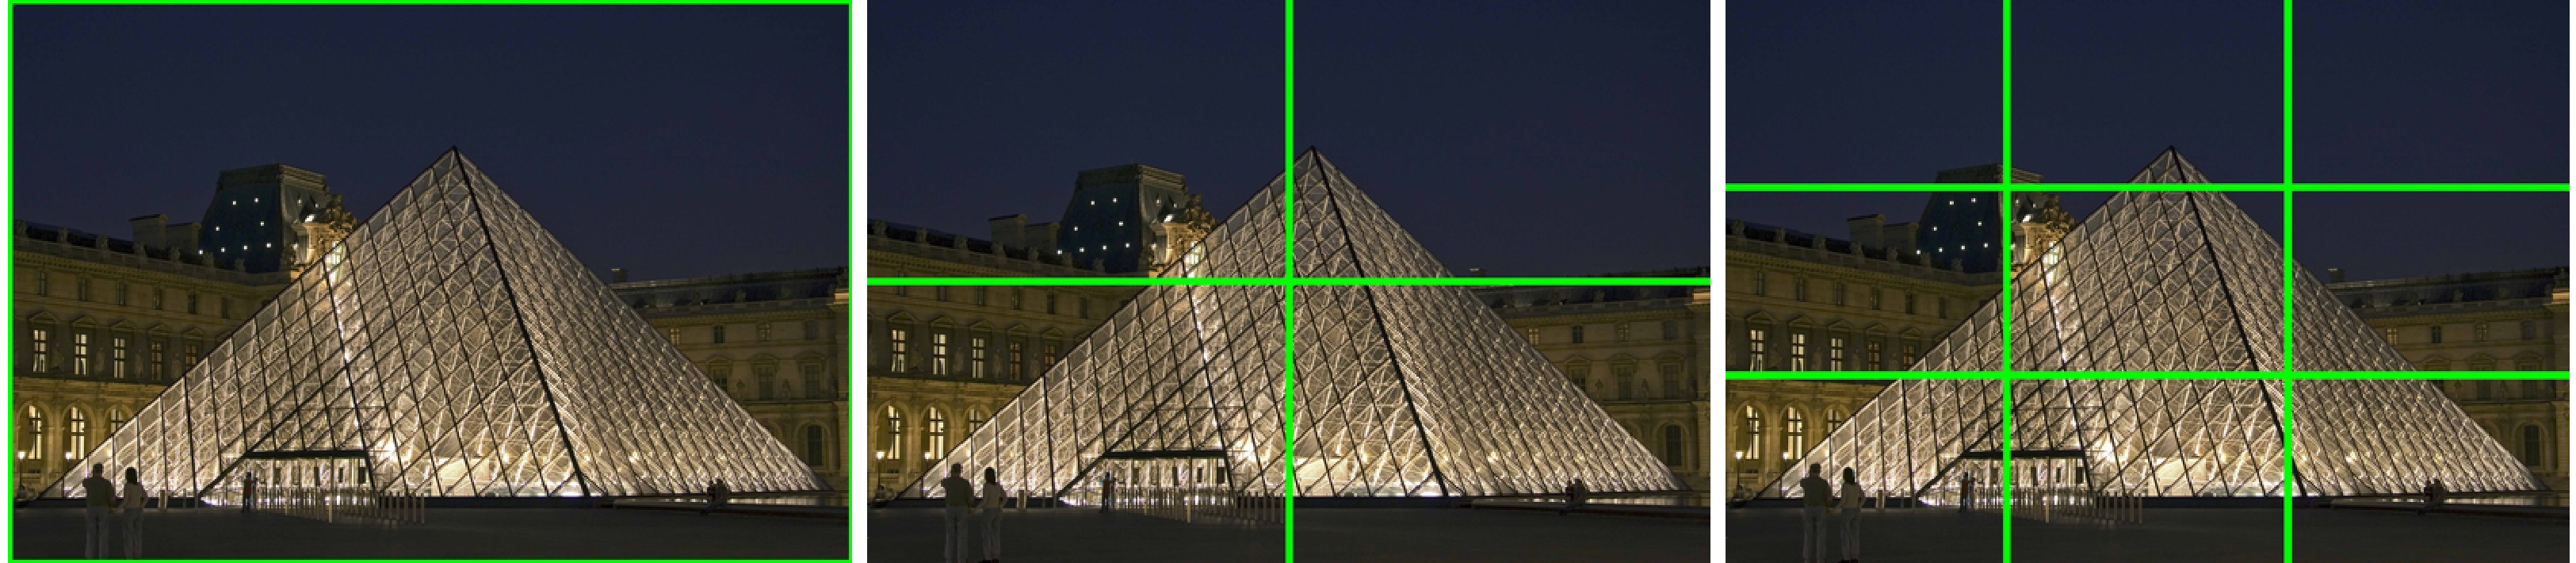
\includegraphics[width=\linewidth]{chapter_mfc_paris_3scale.pdf}
	\caption{图像的 3 尺度特征表示}
	\label{fig:img_multiscale_feature}
\end{figure}

\subsection{多尺度特征表达}\label{subsec:multiscale_img_repr}
不同于 SIFT~\cite{Lowe2004DistinctiveIF}等局部特征描述子,从神经网络提取的特征向量是全局描述子,编码的是图像的全局信息,因此得到的图像特征和图像的语义上的类别关系紧密但是缺乏一些局部以及细节信息,这些细节信息正是评价图像相似性所需要的。受一些多尺度图像特征表达工作~\cite{Lazebnik2006BeyondBO,He2014SpatialPP}的影响,我们试图把这种有效的特征表达方式与合适的图像尺寸改变策略结合在一起,得到具有区分性的特征。在我们的方法中,一张图像由 $L$ 个不同尺度的图像特征金字塔表示,在每个尺度,图像被分为多个互相重合或者不重合的区域,图~\ref{fig:img_multiscale_feature}展示了一张图像 3 尺度表示的示意图。然后我们计算每个小区域的特征表达,并把来自同一尺度的局部特征表达结合起来形成每个尺度的特征。最后我们把每个尺度的特征结合起来,$l_2$ 归一化作为图像最后的特征。

我们试验了三种不同的用来结合局部特征以及不同尺度特征的方法。第一种方法和 He 等提出的空间金字塔~\cite{He2014SpatialPP}相似,来自不同尺度的所有区域特征被 $l_2$ 归一化,然后被拼接成一个特征向量,因此该向量的维度很高,为 $N\times C$,其中 $N$ 是所有来自不同尺度的小区域的个数,$C$ 是特征通道的个数。第二种方法中,区域特征求和并被归一化以后形成尺度级别的特征,然后尺度级别的特征被拼接起来形成图像特征,因此这个特征的维度为 $L \times C$,其中 $L$ 代表尺度的个数。在第三种方法中,区域级别的特征被加起来,然后归一化形成尺度特征,然后尺度特征随即被求和、归一化形成图像的特征表达,图像特征维度为 $C$(特征通道的个数)。

如何有效计算图像各区域的特征也是需要考虑的问题,如果我们将每个图像小块分别送入神经网络来提取特征,计算一张图像特征需要消耗大量的时间,这对于图像检索应用是不现实的。受 ROIpooling~\cite{Ren2017FasterRT}以及 R-MAC(regional maximum pooling of activations) 方法~\cite{Tolias2015ParticularOR}启发,如果我们假设图像区域与特征图对应区域是线性映射关系,那么我们就可以有效地计算图像区域特征,而不用把图像小块重新输入网络。在实验部分,我们实验了不同的提取多尺度特征的设置,报告不同设置得到的特征的检索性能并给出我们的分析。

\subsection{特征降维与白化}
主成份分析法(PCA)是一种常用的有效的特征降维方法,该方法可以使特征的各个分量之间相互独立,白化(whitening)则是使得特征均值为 0,方差为 1。之前的工作~\cite{Babenko2014NeuralCF}已经表明经过 PCA 和 白化以后,特征的检索效果将会提高。在本章中,我们也给出我们的一些发现。

\section{实验}\label{sec:mfc_experiment}
\subsection{实现细节}
我们使用开源深度学习框架 Caffe~\cite{Jia2014CaffeCA}来进行我们所有的实验。我们使用的模型是非常流行的 VGG19 模型~\cite{Simonyan2014VeryDC},该模型是在 ImageNet~\cite{Russakovsky2015ImageNetLS} 分类数据上训练得到的。在实验中,我们使用的特征图来自于网络的最后一层卷积层的输出。

由于原有的 VGG 模型只能接受固定大小的图像输入,这种方式对于需要提取图像特征的检索任务来说,并不是最好的方式。为了使网络能够处理各种大小与长宽比的图像并且测试我们提出的图像尺寸改变的策略,我们把网络变成了全卷积的网络,使得网络能够接受任何大小与长宽比的图像。

\subsection{评价指标与数据库}

\noindent\textbf{(1)评价指标}

图像检索领域两个最基本的指标是准确率(precision)与召回率(recall),准确率指的是返回的结果中,有效的样本占所有返回结果的比例,随着返回结果的增多,准确率通常会降低,常用的还有前 K 个返回结果的准确率,用 precision@k 表示;召回率则指的是返回的结果中,有效的样本占所有有效样本的比例,随着返回结果的增多,召回率通常会上升,同样地,研究者也常使用前 K 个返回结果的召回率,用 recall@k 表示。准确率与召回率是考虑系统性能的两个重要指标,一般来说,准确率高的时候,召回率会比较低,而召回率高的时候,准确率通常又比较低(极端情况就是返回所有的样本,召回率 100\%,但是准确率很低),因此一个好的检索方法必须同时在准确率与召回率上都取得较好的结果,在两个指标上取得平衡。

对于单个查询来说,为了综合反映检索算法的性能,通常并不单独使用准确率和召回率,二是使用综合性的指标,最常使用的一个指标是平均准确率(average precision,简称 AP),该指标同时考虑准确率与召回率,实际上计算的是准确率-召回率曲线下面的面积,用公式表示该指标如下:

\begin{equation}\label{eq:average_prec}
AP = \sum_{k=1}^{n}P(k)\Delta r(k)
\end{equation}

公式\ref{eq:average_prec}中,$P(k)$ 代表 precision@k,$\Delta r(k)$ 代表从 $k-1$ 到 $k$,召回率的变化。

评价检索算法在某个数据库上的性能,常用的评价指标是 mean average precision(简称 mAP),该指标指的是一个数据库上所有查询对应的平均准确率(AP)的均值,用公式表示如下:

\begin{equation}\label{eq:mean_avg_prec}
\text{mAP} = \frac{\sum_{q=1}^{Q}AP(q)}{Q}
\end{equation}

公式~\ref{eq:mean_avg_prec} 中,$AP(q)$ 代表某个查询 $q$ 对应的平均准确率,$Q$ 代表所有查询的数目。

\noindent\textbf{(2)数据库}

在本章的实验中,我们总共使用了四个数据库,现对这四个数据库以及对应的评价指标做一简要介绍:
\begin{enumerate}
\item \textbf{Oxford5k} 数据库~\cite{Philbin2007ObjectRW} 包含了 5062 张从 Flickr 上抓取的 Oxford 建筑图片。该数据库总共包含 55 个查询图像,每个查询图像包含有具体查询区域的坐标,在实验中对于每一幅查询图像,我们使用了两种查询,分别是 \emph{full-query}(使用整个查询图像) 和 \emph{cropped-query}(使用坐标指定区域内的图像)。在该数据库上的评价指标为 mAP。


\item \textbf{Paris6k} 数据库~\cite{Philbin2008LostIQ} 包含了 6412 张来自巴黎的建筑图片\footnote{按照惯例,该数据有 20 张被损坏的图片被去掉,因此实际图片数量是 6392。}。与 Oxford5k 数据库类似,该数据库也包含了 55个 查询图像,同时附带每个图像对应的感兴趣区域的坐标。在这个数据库上的评价指标是 mAP。

\item \textbf{Oxford105k} 数据库包含了的是 Oxford5k 数据库的图片以及额外 100,000 张来自 Flickr 的图片\footnote{有一张损坏图片 \verb+oxc1_100k\portrait\portrait_000801.jpg+ 被移除}~\cite{Philbin2007ObjectRW}。这 100000 张
图片与 Oxford5k 没有相同的图片,被用来作为干扰图片,主要是为了验证数据库规模扩大时的算法的性能。在这个数据库上的评价指标与 Oxford5k 完全一致。

\item  \textbf{UKB} 数据库~\cite{Nistr2006ScalableRW} 总包含了 2550 个物体的 10200 张照片,每个物体 4 张照片。实验时,每张图片被用作查询图片去查询其他图片(包含该图片本身),在这个数据上的评价指标比较特殊,用返回的前四张图片与查询图片相似的平均数目来衡量,是区间 $[0,4]$ 上的一个数,也就是 $4\times recall@4$。

\end{enumerate}

\subsection{实验结果与分析}
在本部分,我们对不同的因素对检索结果影响进行了详细的实验,并给出相应的分析。

\noindent\textbf{(1)图像尺寸变化对检索的影响}

我们对\ref{subsec:img_resize_strategy}节给出的三种图像尺寸变化的策略进行了实验,对于 \emph{two-fixed} 和
\emph{one-fixed} 策略,由于图像的尺寸可以选择多种,我们使用网格搜索来找到性能最好时对应的图像尺寸。我们发现,总体来说,增加图像的尺寸,对于 \emph{full-query} 或者 \emph{cropped-query} 这两种情况,都会提升检索的效果,试验结果如表~\ref{table:image_size_impact}所示,表中括号后面的数字表示取得最好的 mAP 时使用的图像尺寸。从表上可以看出,对于 \emph{cropped-query} 这种情况,\emph{free} 策略能够有效地提升检索的性能,对于 \emph{full-query},\emph{free} 与 \emph{one-fixed} 策略则比较接近,但检索的效果都要好于 \emph{two-fixed} 策略。我们可以看出 \emph{one-fixed} 策略此时要稍高于 \emph{free} 策略,但是 \emph{one-fixed} 情况下,图像最小的边长度被固定在 800,这种设置将大大增加提取特征所需要的计算时间,因为数据库中大部分图像最小尺寸都要小于 800(在表~\ref{table:min_size_distribution} 中,我们列出不同数据库中的图像最小边尺寸的统计信息)。采用 \emph{free} 方式,我们减少特征提取提取时间,并且能够取得很好的检索结果。

实验表明,改变图像的长宽比 (对应 \emph{two-fixed} 策略)对图像信息的干扰最大,因此检索的精度有明显的下降。\emph{one-fixed} 策略虽然没有改变图像的长宽比,但是由于图像尺寸的变化,仍然有一部分信息的丢失。\emph{free} 方式能够编码图像未经扭曲与破坏的信息,因而得到的特征效果更好,能够取得更好的检索结果。

\begin{table}[!t]
	\centering
	\caption{不同图像尺寸变化策略之间的比较}
	\label{table:image_size_impact}
	\begin{tabular}{lll}
		\toprule
		方法		    & full-query			& cropped-query \\
		\midrule
		\emph{two-fixed}		&		55.5 (864)		& 	38.7 (896)	\\
		\emph{one-fixed}		&		59.0 (800) 		&	39.3 (736)\\
		\emph{free}				&		58.0	 		&	52.6 	\\
		\bottomrule
	\end{tabular}
\end{table}

\begin{table}[!t]
	\centering
	\caption{不同数据库中图像最小尺寸落在各个区间的比例($s$ 代表最小尺寸)}
	\label{table:min_size_distribution}
	\begin{tabular}{llll}
		\toprule
		Dataset & $s\leq 500$ & $500<s\leq 800$&  $s>800$ \\
		\midrule
		Oxford5k & 0.87 & 96.86 & 2.27 \\
		Paris6k & 1.30  & 95.59 & 3.11 \\
		Flickr100k & 1.49 & 93.91 & 4.60\\
		UKB & 100 & 0 & 0 \\
		\bottomrule
	\end{tabular}
	\end{table}

\noindent\textbf{(2)图像的多尺度特征表达}

首先我们通过实验比较了 \ref{subsec:multiscale_img_repr}~节提出的区域特征以及尺度特征融合策略,实验结果表明前两种特征融合策略效果不如第三种策略。如果使用第一种策略,检索效果比第三种策略要低 41\%。同时,使用前两种方法得到的图像特征维度(维度至少为 1500 维)也要高于第三种策略(特征维度为 512 维)。高纬度特征也会使得检索时间变长,综合考虑这些,我们采用第三种方式来融合不同的特征。

我们进行了大量实验来确定多尺度方法最好的配置,实验结果列于表~\ref{table:multiscale_exp_result}中。在表中,「overlap」用来指示每个尺度的各个图像区域是否有重叠部分,「s2」和「s3」表示重叠发生了尺度 2 和 3。「weighing」表示各个尺度特征融合的时候,是否采用了不同的权重或者相同的权重。「version」则表示每个尺度使用不同数目的图像块。
\begin{table}[!t]
	\centering
	\caption{不同设置下多尺度特征检索结果对比}
	\label{table:multiscale_exp_result}
	\begin{tabular}{@{}lllllll@{}}
		\toprule
		&   scale &  overlap   &  weighing  & version &     full    &    cropped    \\
		\midrule
		(a1) &   2   & \texttimes & \texttimes &    -    &     63.5      &     59.0      \\
		(a2) &   2   & \texttimes & $\checkmark$ &    -    &     63.9      &     61.0      \\
		\midrule
		(b1) &   3   & \texttimes & \texttimes &    -    &     64.2      &     60.9      \\
		(b2) &   3   & \texttimes & $\checkmark$ &    -    &     62.6      &     61.0      \\
		(b3) &   3   &     s2     & \texttimes &    -    &     64.8      &     60.8      \\
		\midrule
		(c1) &   4   &     s3     & \texttimes &   v1    &     65.1      &     61.4      \\
		(c2) &   4   &     s3     & $\checkmark$ &   v1    &     64.8      &     60.7      \\
		(c3) &   4   &   s2,s3    & \texttimes &   v1    &     65.5      &     60.8      \\
		(c4) &   4   &   s2,s3    & \texttimes&   v2    &     65.9      &     61.5      \\
		(c5) &   4   &   s2,s3    & $\checkmark$ &   v2    &     65.4      &     61.2      \\
		(c6) &   4   & \texttimes & \texttimes &   v3    &     64.5      &     61.3      \\
		(c7) &   4   &     s3     & \texttimes&   v3    &     65.8      &     62.2      \\
		(c8) &   4   &   s2,s3    & \texttimes&   v3    & \textbf{66.3} & \textbf{62.6} \\
		\bottomrule
	\end{tabular}
\end{table}

首先,我们研究了尺度的个数对检索精度的影响。当使用的尺度数目分别为 2 和 3 时,我们使用的每个尺度的区域数目分别为 $\{1\times1, 2\times2\}$ 和
$\{1\times1, 2\times2, 3\times3\}$。对于尺度为 4 的情况,我们使用三种不同版本的区域数目:对于「v1」,「v2」以及「v3」,所使用的图像区域数目分别为 $\{1\times1, 2\times2, 3\times3, 4\times4\}$,$\{1\times1, 2\times2, 3\times3, 5\times5\}$ 和 $\{1\times1, 2\times2, 3\times3, 6\times6\}$。表~\ref{table:multiscale_exp_result} 中 (a1)、(b1)、(c6) 三行列出了分别使用 2, 3, 4 个尺度表示数据图像特征得到的检索结果。很显然,尺度数目的增加也使得检索结果性能变好,特别是对于\emph{cropped-query},检索的结果提高了 3.9\%。

接着,我们也研究给不同的尺度的特征加权融合是否会提升检索的效果。我们使用的不同的尺度的特征加权融合方式类似空间金字塔匹配方法~\cite{Lazebnik2006BeyondBO},也就是说,给来自粗糙尺度上特征更少的权重,给来自精细尺度的特征更大的权重。假设当前总共有 $L$ 个尺度,对应的特征为 $f^1, f^2, \ldots, f^L$,则图像特征 $f$ 计算方式为:

\begin{equation}
f = \frac{1}{2^{L-1}}f^1 + \sum_{i=2}^{L}\frac{1}{2^{L-i+1}}f^i\, .
\end{equation}
关于空间金字塔匹配方法更多的细节,可以参见 Labebnik 等的论文~\cite{Lazebnik2006BeyondBO}。比较 (a1) 和 (a2) 行的结果,看起来似乎加权的方式可以提升检索的性能。我们做了更多的实验,发现随着尺度数目的提高,加权方式来求图像特征并不能提高检索的性能,反而得到了更差的结果,例如,比较 (b1)(b2) 两行的结果,或者比较 (c1)(c2) 两行。这里的结果表明,深度学习提取的特征和传统的特征描述子不同。因此当我们使用对传统的 SIFT 特征有效的方式时,应该有所警惕~\cite{Babenko2015AggregatingLD}。基于这里的实验结果,我们在计算图像特征时,不使用权重不同的策略。

最后,我们研究了同一尺度下不同图像区域重叠(overlapping)是否会提高检索的结果。对于不同尺度数目,我们在一个或者两个尺度下使用重叠的策略。对于行 (b1)(b3) 和 (c1)(c3),我们观察到使用重叠的方式提高了 \emph{full-query} 情况下的结果,但是却降低了 \emph{cropped-query} 情况下的结果。但是对于尺度数目为 4 ,版本是「v3」的情况(比较 (c7)(c8)),我们可以观察到对于 \emph{full-query} 和 \emph{cropped-query},检索结果都有所提高。因此计算最终的图像特征时,我们在尺度 2 和 3 使用了重叠的策略。


\begin{figure}[!t]
	\centering
	\begin{subfigure}{.5\columnwidth}
		\centering
		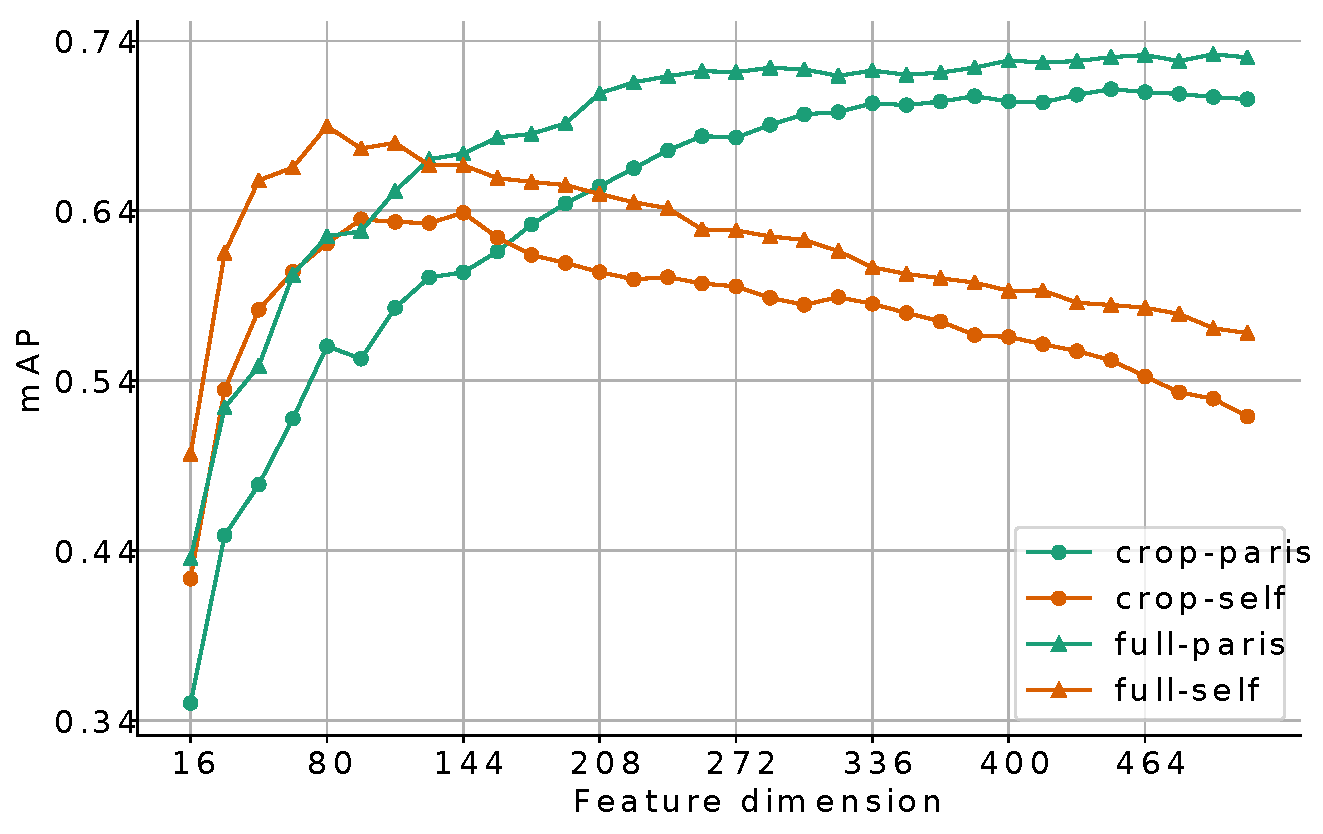
\includegraphics[width=\linewidth]{chapter_mfc_oxford_pca_other_self.pdf}
		\subcaption{Oxford5k}
	\end{subfigure}%
	\hfill
	\begin{subfigure}{.5\columnwidth}
		\centering
		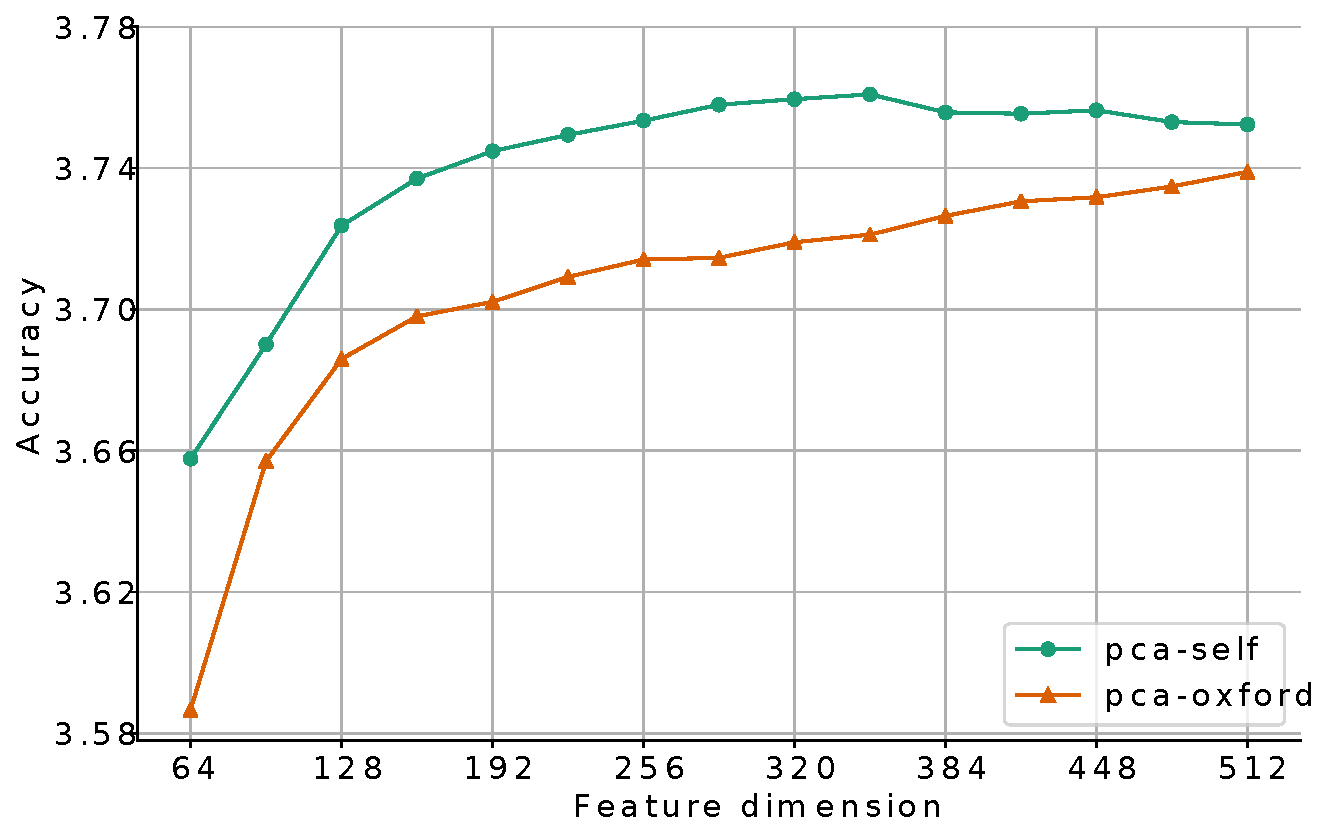
\includegraphics[width=\linewidth]{chapter_mfc_ukb_pca_other_self.pdf}
		\subcaption{UKB}
	\end{subfigure}
	\caption{学习 PCA 与白化矩阵的方式对不同数据库检索结果的影响}
	\label{fig:pca_self_other_exp}
\end{figure}

\noindent\textbf{(3)主成份分析与白化方法}

我们在 Oxford5k 以及 UKB 数据库上进行了 PCA 与白化对检索影响的实验。对于 Oxford5k 数据库,我们分别从 Oxford5k 数据库本身(我们称为「pca-self」)或者从 Paris6k 数据库(我们称为「self-paris」)学习 PCA 与白化矩阵;对于 UKB 数据集,PCA 与白化矩阵则从 UKB 本身(称为「pca-self」)或者从 Oxford5k 上(称为「pca-oxford」)学习得到。我们发现,对于 Oxford5k 数据库,如果从 Paris6k 上学习 PCA 与白化矩阵,检索结果将会提高。但是 UKB 数据库,由于它和 Oxford5k 数据库和 Paris6k 数据库风格不同,从 Oxford5k 数据库学习到的 PCA 与白化矩阵反而对检索结果有害。图~\ref{fig:pca_self_other_exp} 清楚展示了这种不同。同时,对于 Paris6k 数据库,我们也有同样的结果,当使用从 Oxford5k 数据库学习到的 PCA 与白化矩阵时,检索的结果也会有所提升。

\subsection{与其他方法的对比} \label{subsec:mfc_compare_soa}
基于前面的实验结果以及我们的对不同影响因素的分析,我们提出了 \textbf{MFC} 方法 --- 一种多尺度全卷积的图像特征表达方法。对于一张图像,我们不对它进行缩放(\emph{free} 的方式),直接输入到神经网络,然后我们从神经网络的最后一层卷积层的输入的特征图的基础上,提取 4 尺度图像特征表达。在多尺度特征表达中,我们使用最大池化处理特征图,并且使用了区域重叠的策略,我们把区域级别的特征加起来形成尺度特征并归一化,然后把各个尺度的特征求和得到图像特征,再一次归一化。之后,我们学习 PCA 与白化矩阵,对图像特征进行降维。对于不同待测数据库,我们用来学习 PCA 和白化矩阵的数据库分别如下:对于 Oxford5k 及 Oxford105k,我们使用的是 Paris6k;对于 Paris6k 和 UKB,我们使用数据库分别是 Oxford5k 以及 UKB。经过 PCA与白化处理的特征,被再一次归一化,得到最终的特征,这个特征用来报告各种方法的性能。

我们把提出的方法与一些主流的方法进行了比较,这些方法都使用了较低维度的特征,并且没有使用复杂的后处理方法,如几何重排序~\cite{Philbin2007ObjectRW}以及查询扩展~\cite{Chum2007TotalRA}。我们使用了不同的特征维度,实验结果见表~\ref{table:mfc_compare_with_soa},「D」代表特征的维度,「full」与「cropped」分别代表 \emph{full-query} 以及 \emph{cropped-query}。和其他方法相比,在不同的特征维度下,我们的方法都取得了不错的结果。

\begin{table}[!t]
	\centering
	\caption{与其他方法的对比}
	\label{table:mfc_compare_with_soa}
	\begin{tabular}{lllllllll}
		\toprule

		\multirow{2}*{方法}   & \multirow{2}*{D} & \multicolumn{2}{c}{Oxford5k} & \multicolumn{2}{c}{Paris6k} & \multicolumn{2}{c}{Oxford105k} & \multirow{2}*{UKB} \\

		\cmidrule(lr){3-4}	\cmidrule(lr){5-6} \cmidrule(lr){7-8}
		 &                  & full & cropped               & full & cropped              & full & cropped                 &                    \\
		\midrule
		Razavian et al. \cite{Razavian2014CNNFO}              & 256              & 58.9 & -                     & 57.8 & -                    & -    & -                       & 3.65               \\
		SPoC \cite{Babenko2015AggregatingLD}                     & 256              & 58.9 & 53.1                  & -    & -                    & 57.8 & 50.1                    & 3.65               \\
		Neural codes\cite{Babenko2014NeuralCF}                   & 512              & 55.7 & -                     & -    & -                    & 52.2 & -                       & 3.56               \\
		R-MAC \cite{Tolias2015ParticularOR}                      & 512              & -    & 66.8                  & -    & 83.0                 & -    & 61.6                    & -                  \\ \midrule
		Ours                                                     & 256              & 72.2 & 68.4                  & 82.5 & 83.4                 & 68.0 & 62.9                    & 3.75               \\
		Ours                                                     & 512              & 73.0 & 70.6                  & 82.0 & 83.3                 & 68.9 & 65.3                    & 3.75               \\
		\bottomrule
	\end{tabular}
\end{table}

\section{相关工作}\label{sec:mfc_related_work}
Labebnik 等人~\cite{Lazebnik2006BeyondBO}提取使用空间金字塔匹配(简称 SPM)来编码图像的空间信息,在该方法中,可以用多个尺度的金字塔来表示一张图像。来自不同的尺度的特征被结合在一起形成图像的特征,在特征融合的时候,来自精细尺度的特征得到了更多的权重,来自粗糙尺度的特征得到了更少的权重。He 等人~\cite{He2014SpatialPP}提出空间金字塔池化方法(简称 SPP),该方法把神经网路最后一层卷积层输出的特征图划分为不同尺度的金字塔,每个尺度下的区域特征,以及各个尺度的特征被拼接在一起,形成了图像的特征。在我们的工作中,我们也探索了这两种方式是否可行,我们发现使用更简单的特征聚合方式反而取得了更好的结果。

本章采用的是直接提取特征不经过微调的方式来提取图像特征,在这方面有一些喝我们的方法相关的工作。Tolias 等人~\cite{Tolias2015ParticularOR}以及 Babenko 等人~\cite{Babenko2015AggregatingLD}提出使用神经网络的最后一层卷积层的输出作为图像特征,他们分别采用了不同的特征池化方式。Tolias 等人还提出使用一种多尺度的特征表达方式,被称为 R-MAC(regional maximum activation of convolutions),特征图被分为 3 个不同的尺度,每个尺度有一些相互重叠的区域构成,每个尺度的区域个数由原图的长宽比决定。在我们的方法里,我们使用了更简单的策略,每个尺度下区域的个数是固定的,区域的大小根据图像长宽比不同而变化。另外这些工作也没有讨论图像尺寸对检索结果的影响以及该如何学习 PCA 和白化矩阵,才能提升检索的性能。

\section{本章小结}\label{sec:mfc_conclusion}
在本章中,我们介绍了所提出多尺度全卷积的图像特征提取方法。前人工作没有详细地探讨各种因素对检索结果的影响,在本工作中,我们对图像尺寸缩放的策略,多尺度提取特征的方式,以及 PCA 和白化矩阵学习这三个重要的因素进行了研究,并进行了大量的实验,分析三个因素对检索的影响,在此基础上提出了我们的多尺度全卷积的图像特征提取方法。我们在四个数据库进行了实验,实验结果也表明我们提出的方法取得了良好的效果。
